\title{}
\author{}
\date{\today}
\abstract{}
\maketitle

\section{Tokenomics}


\subsection{Token Launch Summary}
Our goal is to raise a minimum of \$5 million USD and a maximum of \$30 million USD. The total number of tokens is capped at \textit{1 billion}. We're currently exploring pricing strategies for the crowd sale. The crowd sale will launch at \textit{\textbf{9AM PST March 15th 2018}}.

\subsection{Token Distribution}
\begin{figure}[htp]
\centering
  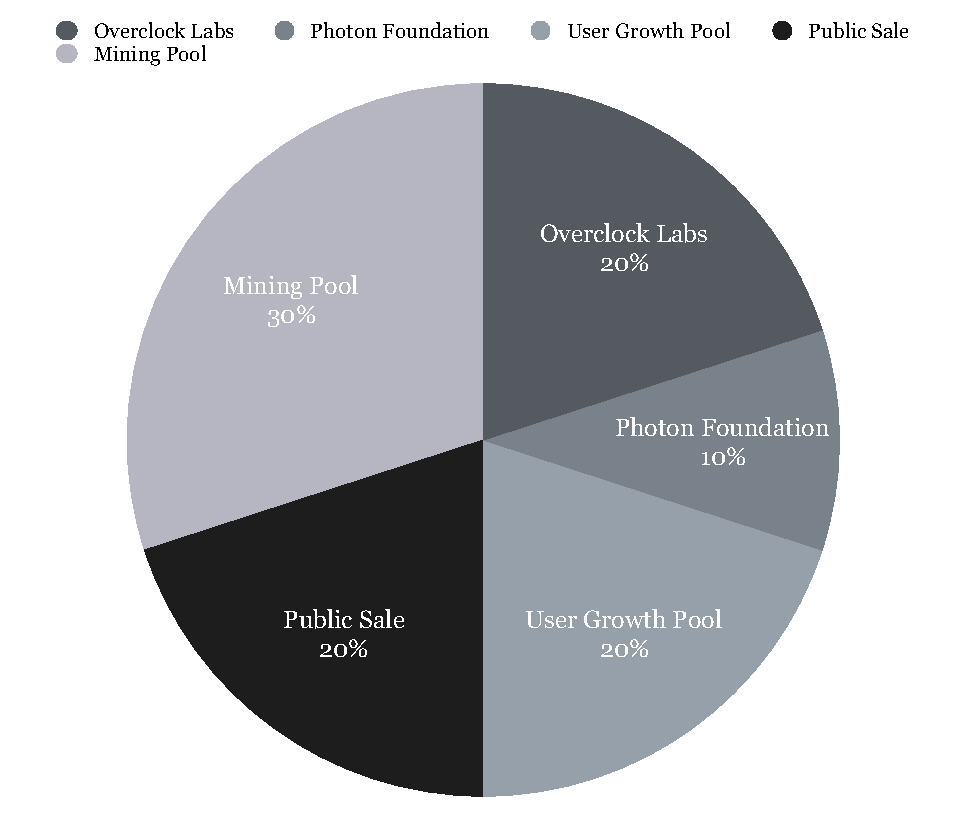
\includegraphics[width=0.5\linewidth]{pool}
  \caption{Photon Token Distribution}
\end{figure}

\begin{itemize}
  \item Overclock Labs: 20\%
  \item Photon Foundation: 10\%
  \item User Growth Pool: 20\%
  \item Public Sale: 20\% 
  \item Mining Pool: 30\%
  \item Token available to public at launch: 200 million 
\end{itemize}

\subsection{User Growth Pool}
The user growth pool is used to incentivize new users to join the Photon Network.                                                                                                   \begin{itemize}
  \item A 200 million endowment is for early adopters of Photon and PHTN of up to 1000 PHTN/user.
  \item PHTN received as a reward can only be used within the PHTN ecosystem for up to 50\% off of services offered.
  \item Unused PHTN after 6 months will be sent back to the user growth fund which can then be used for new users.
  \item No new tokens will be created once the user growth pool is exhausted.
\end{itemize}

\subsection{Budget Allocation}
The majority of the budget 1 focuses on getting the Photon Network off the ground with necessary services, with some room for error and a small marketing budget.    

\begin{figure}[htp]
\centering
  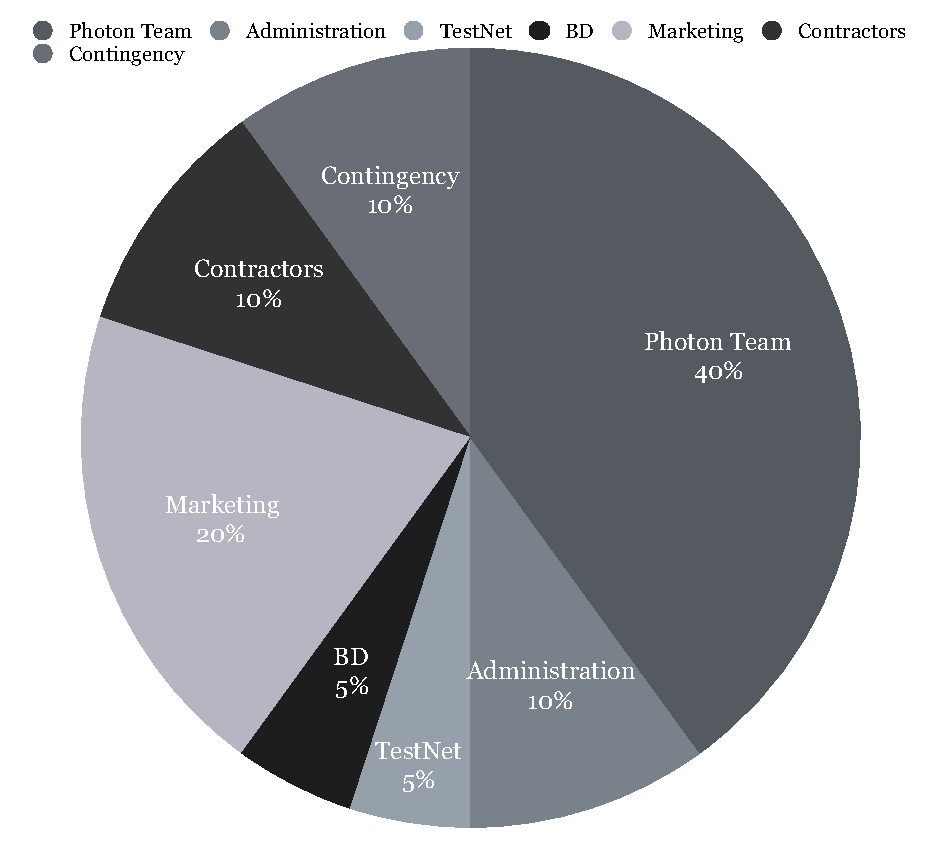
\includegraphics[width=0.6\linewidth]{budget}
  \caption{Budget Allocation}
\end{figure}                                                                          

\begin{itemize}
	\item \textbf{Photon Team: 40\% of budget} The Photon team will consist of just under 30 engineers. This financing allows for the rollout of the Photon Network, Photon Marketplace, including necessary adjustments to and development of the existing Photon Network and Photon Services. 
	\item \textbf{Administration: 10\% of budget} Consists of Photon legal, security, accounting, and other associated administration costs.
	\item \textbf{TestNet: 5\% of budget} Consists of free services provided to our test net users both during our beta test and afterwards, as a reward for helping us solve initial problems on the network.
	\item \textbf{BD Partnerships: 5\% of budget} Consists of funds reserved for integrating, incentivizing, and onboarding channel partners on the the Photon Network.
	\item \textbf{Marketing: 20\% of budget} Marketing will focus on expanding awareness and adoption of the Photon Network among datacenters, providers, clients. Our focus on budget 1 is focused on the US 
	\item \textbf{Contractors: 10\% of budget} These funds will be directed at third-party providers offering engineering, marketing, growth-hacking, PR, partnerships, affiliate programs and more.
	\item \textbf{Contingency: 10\% of budget} This is a set-aside for unforeseen costs.
\end{itemize}	